\documentclass{llncs}
\usepackage{graphicx,wrapfig,url}

\usepackage{listings}
\usepackage{float}
\usepackage{blindtext}
\usepackage{fancyhdr}
\usepackage{fancyhdr}
\usepackage{hyperref}
\usepackage [english]{babel}
\usepackage [autostyle, english = american, maxlevel=4]{csquotes}
\MakeOuterQuote{"}
\usepackage[style=numeric, backend=biber]{biblatex}
%\addbibresource{bibliography.bib}
\floatstyle{ruled}
\pagestyle{plain}
%\usepackage[onehalfspacing]{setspace}



\date{}

\title{Multimedia Databases}
\subtitle{Milestone 4}


%WENIGER FANCY
\author{Deml Miriam (67690) \and Pleyer Wenzel (64682) \and Rotondo Caterina (68391) \and Stemp Christoph (68525)}
\institute{}

\begin{document}


\maketitle

\section{Rationale behind design decisions}
Our frontend is based on the Spring framework in combination with thymeleaf. The HTML itself contains only the necessary functions: the possibility to upload an image and an area for twelve similar images. The search results are retrieved using SQL within a JAVA class (Spring framework). The Oracle database then calls a REST web service, which checks for images and returns the twelve most similar ones including a percentage. Finally the images and their similarity percentage are displayed in the frontend. 

\section{Demonstration results}
This was the chosen example image (9807.jpg):
\begin{center}
	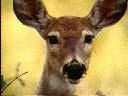
\includegraphics{images/9807.jpg}
\end{center}

\newpage

This is the landing page:
\begin{center}
	
\includegraphics[width=10cm]{images/landing.png}
\end{center}

This is the result page:
\begin{center}
	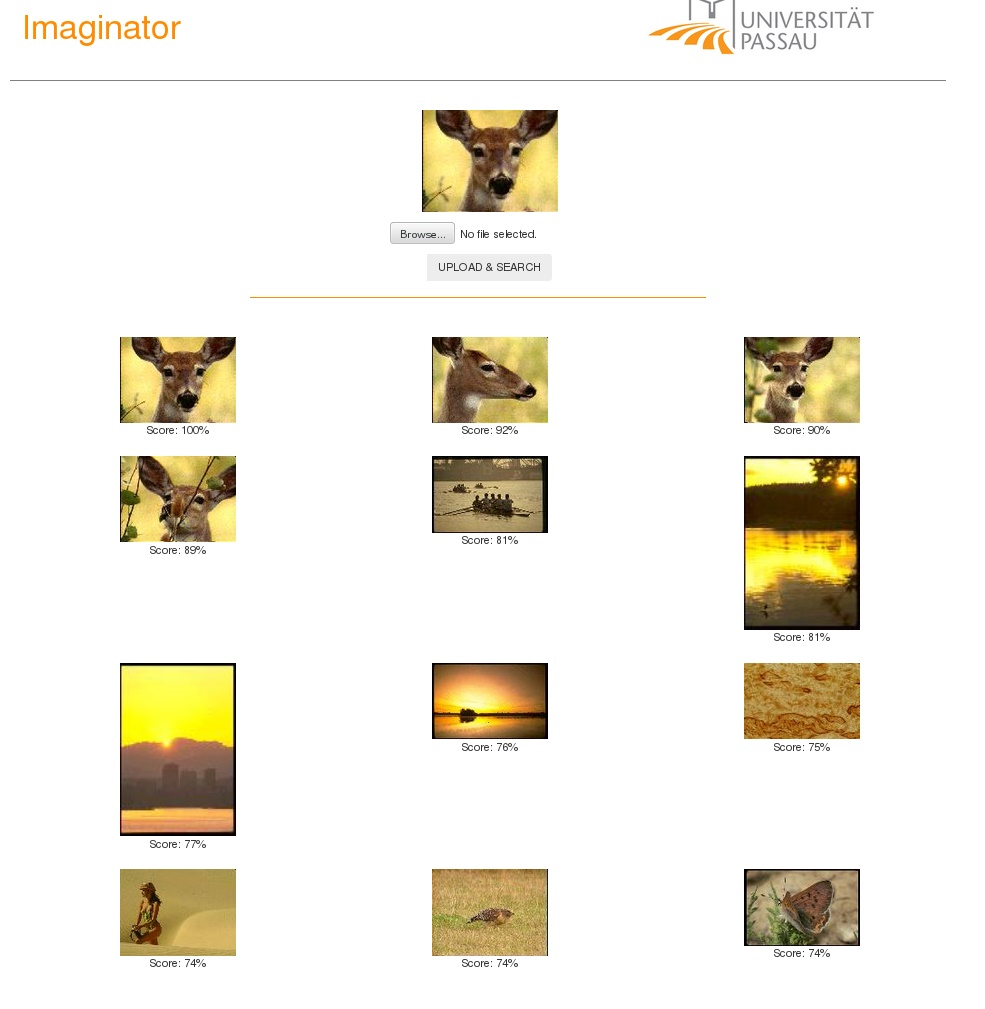
\includegraphics[width=10cm]{images/results.jpg}
\end{center}
%\begin{abstract} 
%\end{abstract}



%\printbibliography

\end{document}